% !TEX root = ./notes_template.tex
%%%%%%%%%%%%%%%%%%%%%%%%%%%%%%%%%%%%%%%%%%%%%%%%%%
%%%%%%%%%%%%%%%%%%%%% preamble %%%%%%%%%%%%%%%%%%%
%%%%%%%%%%%%%%%%%%%%%%%%%%%%%%%%%%%%%%%%%%%%%%%%%%
\documentclass[11pt,twoside]{book}
\usepackage[mono=false]{libertine} % new linux font, ignore mono

\usepackage{luatex85}

%\renewcommand{\baselinestretch}{1.05}
\usepackage{amsmath,amsthm,amssymb,mathrsfs,amsfonts,dsfont}
\usepackage{epsfig,graphicx}
\usepackage{tabularx}
\usepackage{blkarray}
\usepackage{slashed}
\usepackage{color}
\usepackage{listings}
\usepackage{caption}
% \usepackage{fullpage}
\usepackage{lipsum} % provides dummy text for testing
\usepackage[toc,title,titletoc,header]{appendix}
\usepackage{minitoc}
\usepackage{color}
\usepackage{multicol} % two-col ToC
\usepackage{bm}
\usepackage{imakeidx} % before hyperref
\usepackage{hyperref}
% link colors settings
\hypersetup{
    colorlinks=true,
    citecolor=magenta,
    linkcolor=blue,
    filecolor=green,      
    urlcolor=cyan,
    % hypertexnames=false,
}
\usepackage{marginnote}
\usepackage[capitalise]{cleveref}
\usepackage{subcaption}
\usepackage{enumitem}
\usepackage{mathtools}
\usepackage{physics}
\usepackage[linesnumbered,ruled,vlined,algosection]{algorithm2e}
\newcommand\mycommfont[1]{\footnotesize\ttfamily\textcolor{blue}{#1}} % https://tex.stackexchange.com/questions/162207/algorithm2e-comment-style
\SetCommentSty{mycommfont}
% \SetCommentSty{textsf}
\usepackage{epigraph}
\epigraphwidth=1.0\linewidth
\epigraphrule=0pt

% adjust margin
\usepackage[margin=2.3cm]{geometry}
\headheight13.6pt

% colored boxes
\usepackage[most]{tcolorbox}

%%%%%%%%%%%%%%%% thmtools %%%%%%%%%%%%%%%%%%%%%
\usepackage{thmtools}
\declaretheorem[numberwithin=chapter]{theorem}
\declaretheorem[numberwithin=chapter]{axiom}
\declaretheorem[numberwithin=chapter]{lemma}
\declaretheorem[numberwithin=chapter]{proposition}
\declaretheorem[numberwithin=chapter]{claim}
\declaretheorem[numberwithin=chapter]{conjecture}
\declaretheorem[sibling=theorem]{corollary}
\declaretheorem[numberwithin=chapter, style=definition]{definition}
\declaretheorem[numberwithin=chapter, style=definition]{problem}
\declaretheorem[numberwithin=chapter, style=definition]{example}
\declaretheorem[numberwithin=chapter, style=definition]{exercise}
\declaretheorem[numberwithin=chapter, style=definition]{observation}
\declaretheorem[numberwithin=chapter, style=definition]{fact}
\declaretheorem[numberwithin=chapter, style=definition]{construction}
\declaretheorem[numberwithin=chapter, style=definition]{remark}
\declaretheorem[numberwithin=chapter, style=remark]{question}
%%%%%%%%%%%%%%%% thmtools %%%%%%%%%%%%%%%%%%%%%
\usepackage{changepage}
\newenvironment{solution}
    {\renewcommand\qedsymbol{$\square$}\color{blue}\begin{adjustwidth}{0em}{2em}\begin{proof}[\textit Solution.~]}
    {\end{proof}\end{adjustwidth}}

%%%%%%%%%%%%%%%% index %%%%%%%%%%%%%%%%%%%%%
\begin{filecontents}{index.ist}
% https://tex.stackexchange.com/questions/65247/index-with-an-initial-letter-of-the-group
headings_flag 1
heading_prefix "{\\centering\\large \\textbf{"
heading_suffix "}}\\nopagebreak\n"
delim_0 "\\nobreak\\dotfill"
\end{filecontents}
\newcommand{\myindex}[1]{\index{#1} \emph{#1}}
\makeindex[columns=3, intoc, title=Alphabetical Index, options= -s index.ist]
%%%%%%%%%%%%%%%% index %%%%%%%%%%%%%%%%%%%%%

%%%%%%%%%%%%%%%% ToC %%%%%%%%%%%%%%%%%%%%%
% Link Chapter title to ToC: https://tex.stackexchange.com/questions/32495/linking-the-section-text-to-the-toc
\usepackage[explicit]{titlesec}
\titleformat{\chapter}[display]
  {\normalfont\huge\bfseries}{\chaptertitlename\ {\thechapter}}{20pt}{\hyperlink{chap-\thechapter}{\Huge#1}
\addtocontents{toc}{\protect\hypertarget{chap-\thechapter}{}}}
\titleformat{name=\chapter,numberless}
  {\normalfont\huge\bfseries}{}{-20pt}{\Huge#1}

%%%%%%%%%%%%%%%%%%% fancyhdr %%%%%%%%%%%%%%%%%
\usepackage{fancyhdr}
\pagestyle{fancy} % enable fancy page style
\renewcommand{\headrulewidth}{0.0pt} % comment if you want the rule
\fancyhf{} % clear header and footer
\fancyhead[lo,le]{\leftmark}
\fancyhead[re,ro]{\rightmark}
\fancyfoot[CE,CO]{\hyperref[toc-contents]{\thepage}}

% https://tex.stackexchange.com/questions/550520/making-each-page-number-link-back-to-beginning-of-chapter-or-section
\makeatletter
\def\chaptermark#1{\markboth{\protect\hyper@linkstart{link}{\@currentHref}{Chapter \thechapter ~ #1}\protect\hyper@linkend}{}}
\def\sectionmark#1{\markright{\protect\hyper@linkstart{link}{\@currentHref}{\thesection ~ #1}\protect\hyper@linkend}}
\makeatother
%%%%%%%%%%%%%%%%%%% fancyhdr %%%%%%%%%%%%%%%%%


%%%%%%%%%%%%%%%%%%% biblatex %%%%%%%%%%%%%%%%%
\usepackage[doi=false,url=false,isbn=false,style=alphabetic,backend=biber,backref=true]{biblatex}
\addbibresource{bib.bib}

\newbibmacro{string+doiurlisbn}[1]{%
  \iffieldundef{doi}{%
    \iffieldundef{url}{%
      \iffieldundef{isbn}{%
        \iffieldundef{issn}{%
          #1%
        }{%
          \href{http://books.google.com/books?vid=ISSN\thefield{issn}}{#1}%
        }%
      }{%
        \href{http://books.google.com/books?vid=ISBN\thefield{isbn}}{#1}%
      }%
    }{%
      \href{\thefield{url}}{#1}%
    }%
  }{%
    \href{http://dx.doi.org/\thefield{doi}}{#1}%
  }%
}

% https://tex.stackexchange.com/questions/94089/remove-quotes-from-inbook-reference-title-with-biblatex
\DeclareFieldFormat[article,incollection,inproceedings,book,misc]{title}{\usebibmacro{string+doiurlisbn}{\mkbibemph{#1}}}
% https://tex.stackexchange.com/questions/454672/biblatex-journal-name-non-italic
\DeclareFieldFormat{journaltitle}{#1\isdot}
\DeclareFieldFormat{booktitle}{#1\isdot}
% https://tex.stackexchange.com/questions/10682/suppress-in-biblatex
\renewbibmacro{in:}{}
% add video field: https://tex.stackexchange.com/questions/111846/biblatex-2-custom-fields-only-one-is-working
\DeclareSourcemap{
    \maps[datatype=bibtex]{
      \map{
        \step[fieldsource=video]
        \step[fieldset=usera,origfieldval]
    }
  }
}
\DeclareFieldFormat{usera}{\href{#1}{\textsc{Online video}}}
\AtEveryBibitem{
    \csappto{blx@bbx@\thefield{entrytype}}{% put at end of entry
        \iffieldundef{usera}{}{\space \printfield{usera}}
    }
}
%%%%%%%%%%%%%%%%%%% biblatex %%%%%%%%%%%%%%%%%

%%%%%%%%%%%%%%%%%%%%% glossaries %%%%%%%%%%%%%%%%%
% !TEX root = ./notes.tex
\usepackage[style=super]{glossaries}
\setlength{\glsdescwidth}{1\linewidth}
\makeglossaries

\renewcommand\glossaryname{List of Abbreviations and Symbols}

\newglossaryentry{Q2}{name={$Q_2(f)$},
%sort=Q2,
description={Two-side (bounded) error quantum query complexity}}
\newglossaryentry{real_number}{name={$\mathbb{R}$},description={Real number}}
%%%%%%%%%%%%%%%%%%%%% glossaries %%%%%%%%%%%%%%%%%

%%%%%%%%%%%%%%%%%%%%% glossaries-extra %%%%%%%%%%%%%%%%%
% \usepackage[record,abbreviations,symbols,stylemods={list,tree,mcols}]{glossaries-extra}
%%%%%%%%%%%%%%%%%%%%% glossaries-extra %%%%%%%%%%%%%%%%%


% !TEX root = ./notes.tex

%%%%%%%%%%%%%%%%%%%%%%%%%%%%%%%%%%%%
%%%%%%%%%%%%%%%%%%%%%%%%%%%%%%%%%%%%
% math
\let\iff\relax
\newcommand{\iff}{\text{ iff }}
\newcommand{\OPT}{\textup{OPT}}

% physics
\newcommand{\acreation}{a^\dagger}



%%%%%%%%%%%%%%%%%%%%%%%%%%%%%%%%%%%%%%%%%%%%%%%%%%
%%%%%%%%%%%%%%%% begin of document %%%%%%%%%%%%%%%
%%%%%%%%%%%%%%%%%%%%%%%%%%%%%%%%%%%%%%%%%%%%%%%%%%

\begin{document}

\title{\bf \huge Metabook}
\author{Leidy-Alejandra G. Molano}
\date{Update on \today}
\maketitle
\setcounter{tocdepth}{2}
\setcounter{minitocdepth}{1} 

\begin{multicols}{2}
    \dominitoc% Initialization
    \adjustmtc[2]% chp number shift for mini-toc
    \tableofcontents
    \label{toc-contents}
\end{multicols}

	\listoffigures
	% \listoftables
\begin{multicols}{2}
	\listoftheorems[ignoreall,show={theorem}]
\end{multicols}

	\renewcommand{\listtheoremname}{List of Definitions}
\begin{multicols}{2}
	\listoftheorems[ignoreall,show={definition}]
\end{multicols}

	% \printglossaries
	% \printglossary[type=\acronymtype]
	\printglossary
	% \printglossary[title=List of terms, toctitle=List of terms]

	% bib2gls
	% \printunsrtglossaries % print all types
	% \printunsrtglossary[type={abbreviations},title=List of Abbreviations,style=listgroup]
	% \printunsrtglossary[type={abbreviations},title=List of Abbreviations,style=listhypergroup] % doesn't work
	% \printunsrtglossary[type={symbols},title=List of Symbols,style=listgroup]
	% \printunsrtglossary % main entry

%%%%%%%%%%%%%%%Content%%%%%%%%%%%%%%%
% \mainmatter % separat the number of toc and mainmatter
% !TEX root = ../notes_template.tex
\chapter{Preface}

\section{Features of this template}

\begin{itemize}
    \item different styles of clickable definitions and theorems
    \begin{itemize}
        \item nameref:
            \nameref{def:gaussian_distribution}

        \item autoref:
            \autoref{def:gaussian_distribution}

        \item cref:
            \cref{def:gaussian_distribution}

        \item hyperref:
            \hyperref[def:gaussian_distribution]{Gaussian}
    \end{itemize}

    \item toc: list of theorems, definitions
    \item bib: titles of reference is linked to the publisher webpage 
        \cite{kitaev2002classical}
        \cite{childsUniversalComputationQuantum2009}
    \item index
    \myindex{index} 
    \item glossary
    \gls{real_number}
\end{itemize}

\begin{figure}[!ht]
    \centering
    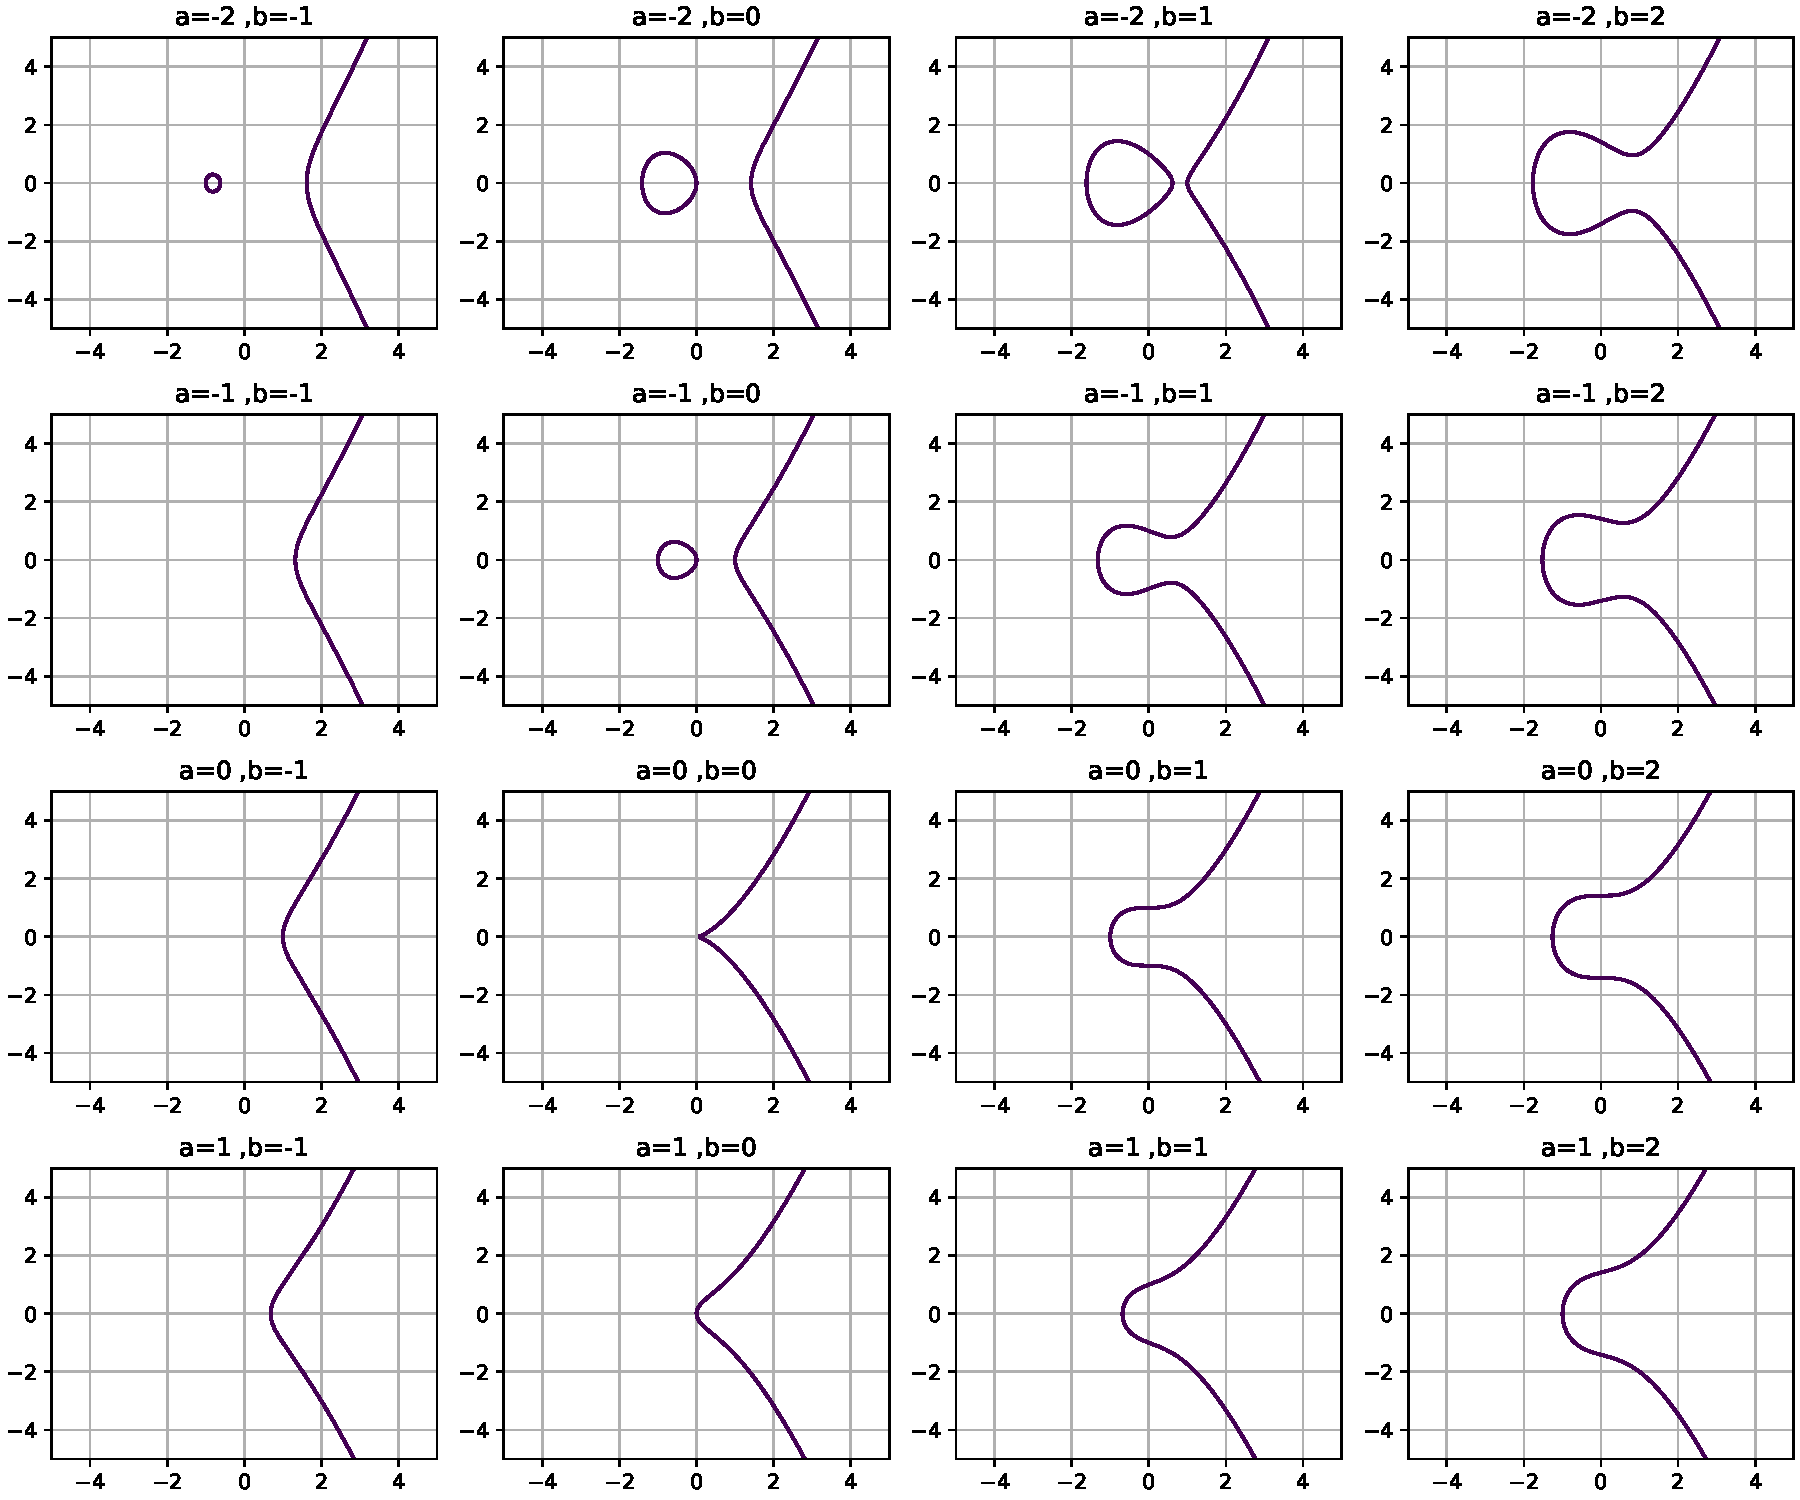
\includegraphics[width=1\linewidth]{./figure/elliptic_curves.pdf}
    \caption{Elliptic curves}
\end{figure}


\part{Genomes}
% !TEX root = ../notes_template.tex
\chapter{Human Genome}\label{chp:human_genome}

\minitoc

gls examples:
\begin{itemize}
	% \item \glsxtrshort{gcd};
	\item \Gls{gcd}; \acrlong{gcd}; \acrshort{gcd}; \acrfull{gcd}
\end{itemize}

\section{Introduction}
\begin{itemize}
    \item 3.2 billion base pairs 
    \item Haploid (n, gametes): 22 autosomal chromosomes + 1 sexual (X or Y).
    \item Diploid (2n, zygote): 46 autosomal chromosomes + 2 sexual (XX, XY). Every gene present in autosomes is present 
    in two copies in the zygote. Then individuals contain two genomes, one maternal and one paternal, which get mixed in 
    the cell nucleus after the first mitotic division.
    \item The total number of protein-coding genes distributed on the 23 chromosomes of the human genome is estimated to 
    be 20,412, slightly less than 20,470 genes of the \textit{Caenorhabditis elegans} \cite{Pena2021} and only the double of one strain of 
    \textit{Ktedonobacter racemifer}, with 11,453 protein-coding genes \cite{He2024}.
\end{itemize}
\begin{figure}[!ht]
    \centering
    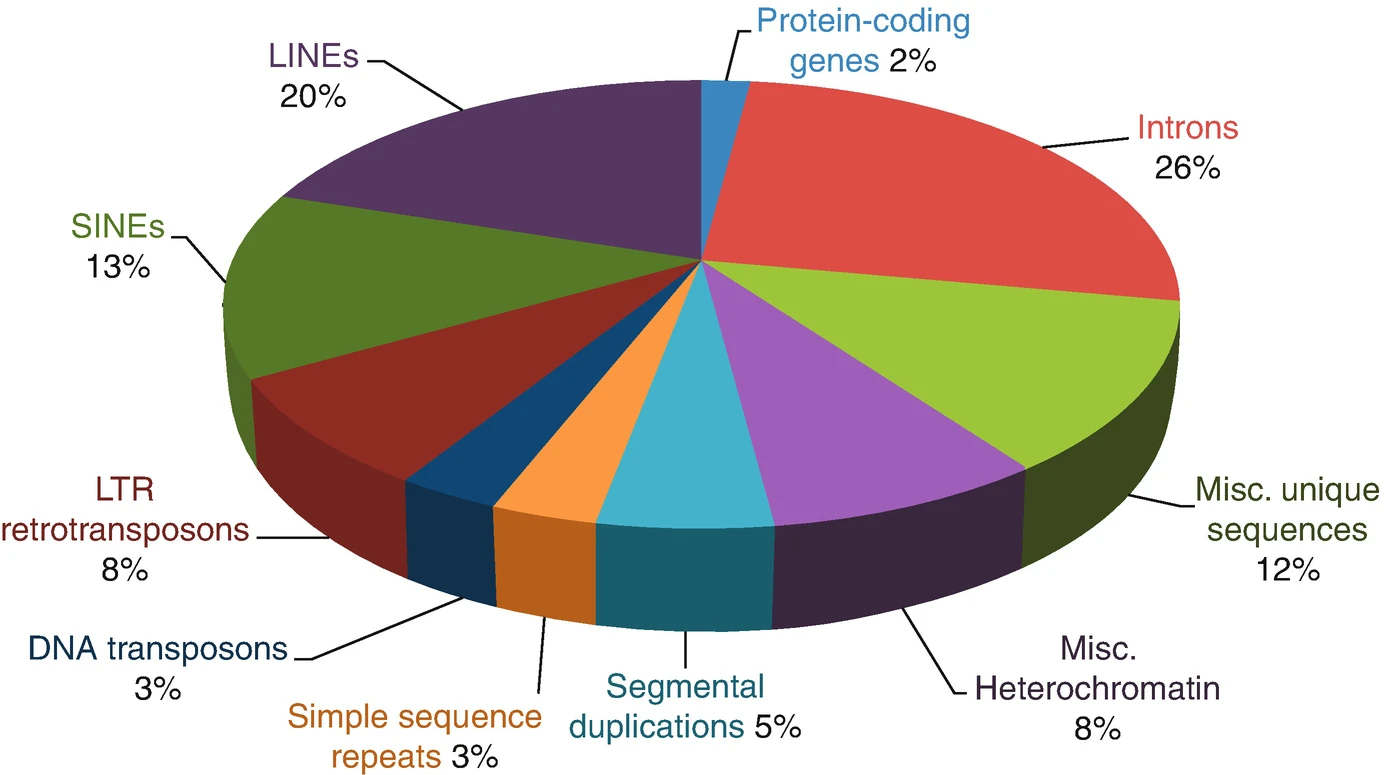
\includegraphics[width=1\linewidth]{./figure/composition_human_genome.png}
    \caption{Composition of the human genome. Redrawn from a graph that was produced in 2014 by the NHS National Genetics 
    and Genomics Education Centre. Borrowed from \citetitle{Pena2021} \cite{Pena2021}}
    \label{fig:composition_human_genome}
\end{figure}

\section{Chromosomes}

Chromosomes are the basic morphological division of the human genome.The number of genes on each human chromosome varies widely, 
from 2058 genes on chr1 to only 71 genes on Y chr. The density of genes on chromosomes also varies widely. For instance, 
chromosome 19 is smaller than chromosome 13, but contains almost four times more genes than the latter 
(chromosome 19 is the second in decreasing order of gene content, just behind the chromosome 1). The three autosomes 
with the fewest genes are chromosome 13 (327 genes), chr 18 (270 genes), and chr 21 (234 genes). It is thus no accident 
that the only autosomal human trisomies compatible with the survival of the fetus till birth are trisomies 13, 18 and 21! 

There is apparently no specific reason why humans have 46 chromosomes in somatic cells. Our closest primate, the chimpanzee 
(\textit{Pan troglodytes}) has 48 chromosomes. In the evolution of primates, two acrocentric chromosomes from the chimpanzee underwent 
centric fusion to form human chromosome 2, hence the reduction of chromosome number to 46. In contrast, the mouse (\textit{Mus musculus}) 
has 56 chromosomes. The \textit{Lysandra atlantica} butterfly has 446 chromosomes in diploid cells, while \textit{Lysandra golga} has 268 and 
\textit{Lysandra nivescens} has 82! In fact, there seems to be no correlation between the number of chromosomes or the size of the 
total genome or the biological complexity of the species. Both seem to vary at random. Thus, everything suggests that the 
chromosomes may be only physical frameworks that allow the realization of mitosis and meiosis in sexual species. 

The chromosomes seem to behave functionally as “packages” of genes. In general, the functioning of individual genes is not 
affected by their chromosomal position. For instance, there are individuals with balanced chromosomal translocations, in 
which chromosomes have exchanged segments without loss or net gain of genetic material—such individuals do not present any 
clinical manifestation of translocation, except perhaps for reproductive difficulties, as some translocations may interfere 
with the production of gametes in meiosis, especially in the male. 

\textbf{Centromere}. In chromosomes, DNA contains genes that are expressed according to the needs of the cell, but it also contains 
specialized sequences that are necessary for intrinsic functions of the chromosome itself. On one hand, chromosomes need 
to be properly aligned during cell division. This requires a centromere, a region where a pair of protein complexes, called 
kinetochores, binds just before the start of cell division. Microtubules are responsible initially for positioning the 
chromosomes correctly in the metaphase and then for pulling the individualized chromosomes to opposite poles of the mitotic 
spindle. The DNA sequences in the centromeres are very different in different organisms. In mammalian chromosomes, centromeric 
DNA is a heterochromatic region, with no informational content, dominated by repetitive DNA sequences that often extend 
monotonously by mega DNA bases. 

\textbf{Telomere}. At the ends of chromosomes, there are specialized structures called telomeres, which are necessary for maintaining 
chromosomal integrity. If a telomere is lost after a break in a chromosome, the resulting chromosomal end is unstable and 
tends to merge with the broken ends of the other chromosomes, or even be degraded. In vertebrate telomeres the DNA consists 
of multiple copies in tandem of the oligonucleotide TTAGGG, sequence at which certain telomeric proteins bind. The repetitive 
units of the telomeres decrease in number with every division of the DNA. As the enzyme needed to regenerate telomeres (telomerase) 
is not available in normal somatic cells, telomeres are a kind of biological clock that records our age.  

\section{Coding and Non-coding DNA}
The vast majority of genes are in the chromosomes of the nucleus; a few are also found in mitochondrial DNA. 

\textbf{Human vs Chimpanzee}. Remarkable similarities of known human and chimpanzee protein sequences initially led to the 
suggestion that significant differences might be primarily in gene and protein expression, rather than protein structure. 
Further analysis of alignable non-coding sequences affirmed this \(\backsim\)1\% difference. However, the subsequent identification 
of non-alignable sequences that were due to segmental deletions and duplications has shown that the overall difference between 
the two genomes is actually \(\backsim\)4\%.  

Less than 2\% of the human genome corresponds to protein-coding genes (\autoref{fig:composition_human_genome}). The functional 
role of the remaining 98\%, apart from repetitive sequences (constitutive heterochromatin) that appear to have a structural 
role in the chromosome, is a matter of controversy. 

\section{Retroposons, Retrotransposons, and Retrovirus}
Transposable elements can be separated into two major classes: 
\begin{itemize}
    \item \textbf{DNA transposons}. Constitute approximately 3\% of the human genome (\autoref{fig:composition_human_genome}; 
    \autoref{fig:human_transposable_elements}), 
    can excise themselves from the genome, move as DNA and insert themselves into new genomic sites. Although DNA transposons 
    are currently not mobile in the human genome, they were apparently active during early primate evolution.
    \item \textbf{Retroposition elements}. i.e. retroposons, retrotransposons and endogenous retroviruses, duplicate through 
    RNA intermediates that are reverse transcribed and inserted at new genomic locations. Together, they constitute more 
    than 40\% of the human genome.
\end{itemize}
\begin{figure}[!ht]
    \centering
    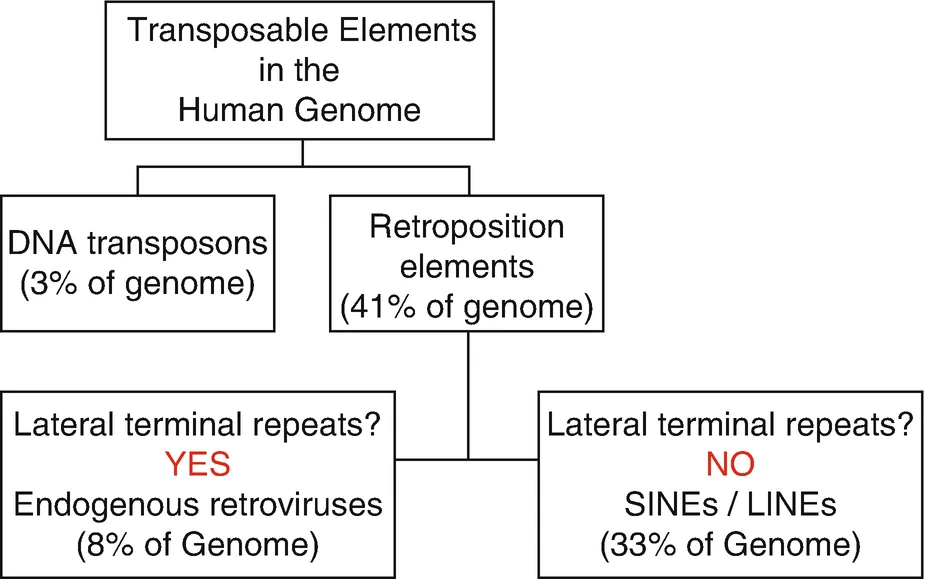
\includegraphics[width=1\linewidth]{./figure/human_transposable_elements.png}
    \caption{Classes of transposable elements in the human genome. Borrowed from \citetitle{Pena2021} \cite{Pena2021}}
    \label{fig:human_transposable_elements}
\end{figure}

\textbf{Retroposons}. Do not contain the gene for reverse transcriptase and thus are dependent on exogenous sources of 
the enzyme (mostly from Long Interspersed Nuclear Element s—LINEs) for retroposition. They share similarity with genes 
transcribed by RNA polymerase III, the enzyme that transcribes genes into ribosomal RNA, tRNA and other small RNA molecules. 
An especially abundant group of retroposons in humans is the Alu family of SINEs (Short Interspersed Nuclear Elements ), 
that basically represents a processed pseudogene of the Signal Recognition Particle (7SL) RNA. The Alu family of retroposons 
(thus called because they contain a site for digestion by the restriction enzyme AluI) makes up 13\% of the human genome. 
Virtually all other mammalian SINEs differ from the human, being derived from tRNA genes.  

\textbf{Retrotransposons}. In contrast, do code for reverse transcriptase and hence are capable of autonomous retrotranscription. 
They also contain a promoter for RNA polymerase II, which allows it to insert itself into random positions. In humans, LINEs, 
which altogether make up 20\% of the human genome, are the main class of retrotransposons. Although the vast majority of 
human LINE-1 sequences are inactive molecular fossils, an estimated 80-100 copies per individual still retain the ability 
to mobilize and expand in numbers within the human genome, by cycles of transcription, retrotranscription and retroposition. 
Some of these active LINEs constitute insertional polymorphisms in the human species. LINEs and SINEs continue growing in 
numbers in all mammalian genomes, and thus are “genomic parasites”, the ultimate “selfish genes”.  

\textbf{Endogenous retroviruses}. The class of retrotransposons that contain lateral terminal repeats (LTRs), which are evolutionarily 
related to the exogenous retrovirus group of RNA virus and will be the focus of this section (\autoref{fig:human_transposable_elements}). 
They constitute around 8\% of the human genome! This is ironic, considering that at the very moment that I am writing this 
chapter humanity is being held ransom by the RNA virus SARS-CoV-2 that causes the serious disease COVID-19. Thus, if not 
only for its timeliness, I think that today any discussion of the structure and function of the human genome should include 
a discussion of these endogenous retroviruses. In special I want to evaluate the evidence for a conceivable anti-viral effect 
of these mostly defective and dormant endogenous retroviruses, which eons ago were exogenous, infected germ cells, endogenized 
and multiplied to become 8\% of the human genome. 

An endogenous retrovirus is generally called ERV or EVE (endogenous viral element). Although not one of the thousands of 
retrovirus-related sequences found in the human genome contains a complete set of intact retroviral genes or can express 
infectious virus, these sequences are nonetheless referred to as Human Endogenous Retroviruses (HERVs). More info in the 
section of An Overview of the Human Genome.
% !TEX root = ../notes_template.tex
\chapter{Prokaryotic Genomes}\label{chp:prokaryotic_genomes}

\minitoc

\section{Introduction}
To be done. Check \citetitle{He2024} \cite{He2024}

\part{Mobile Genetic Elements}
Mobile genetic elements (MGEs) are selfish genetic entities that are unable to self-replicate and rely on host cells and 
cellular machinery to propagate. They can move around within a genome or be transferred across species.

% !TEX root = ../notes_template.tex
\chapter{Plasmids}\label{chp:Plasmids}

\minitoc
 

\section{Introduction}
Plasmid are DNA molecules located outside of the chromosomal DNA, i.e. extrachromosomal. Their topology is frequently 
circular although linear plasmid also exists. They have been extensively studied in Bacteria, even though Archaea and 
Eukaryota also carry them. 

Plasmids are generally associated with a host range, which can be broad or narrow. Incompatibility groups used from plasmid 
classification. Seems that their host range is determined by their ability to escape host defenses and the use of host's machinery. 

Mainly, plasmids mobility has been associated to its conjugation system, although other mechanisms have been described, 
such as membrane vesicles (castañeda 2024). Importantly, not all plasmids have transfer and mobility functions. 

Due to their mobility, plasmids are included in the category of mobile genetic elements, along with 
Integrative Conjugative Elements (ICEs, which integrate into the host genome and carry a functional conjugation system for 
inter-cellular transfer, \(\backsim\)18-500 kb in length) and phages (forming viral particles that infect a prokaryotic cell, 
replicating within it and are transferred between the cells via transduction, \(\backsim\)11-500 kb in length) (Khedkar 2022). 

Insertion sequences (IS, elements carry only a transposase gene, \(\backsim\)2.5 kb in length) and, transposons (elements 
that carry transposase and dispensable cargo genes, \(\backsim\)5 kb in length) and integrons (gene acquisition systems 
that are immobile without other MGEs, several kb in length) depend on other MGEs for inter-cellular transfer.

\section{Structure}
\begin{itemize}
    \item \textbf{Backbone}. Consists in two differentiated parts.
    \begin{itemize}
        \item Essential genes that ensure vertical inheritance (replication, copy number, partitioning, stability).
        \item Inessential genes that code for horizontal gene transfers.
    \end{itemize}
    \item \textbf{Genetic cargo}. Regions outside backbone that may contribute a phenotypic advantage to their hosts. 
\end{itemize}
Plasmid stability depends on the balance between genetic burden and beneficial effect to the host (genetic cargo).

\section{Replication}
The fundamental characteristic that defines a plasmid is its ability to replicate autonomously. This independence allows 
the plasmid to present a copy number higher than the chromosome. 
\begin{align*}
    Plasmid\ copy\ number = \frac{\#\ plasmid}{\#\ chromosomal\ copies} 
\end{align*}

However, they also seem to replicate in step with the chromosome, doubling in number during the cell growth of their host, 
being vertically inherited from generation to generation. Plasmids use at least three distinct types of replication systems: 
rolling circle, theta, and linear replication. \textbf{Rolling circle} is generally confined to small and high copy number 
plasmids, whereas large and low copy number plasmids invariably use types of \textbf{theta} or \text{linear} replication systems. 

Plasmids are replicons that transfer between cells via conjugation (6), up to 2.5 Mb in length. This independence from the 
chromosome defines them as genetic locus where genes may evolve faster than in the chromosome.

\section{Toxin-Antitoxin systems}
Many bacteria encode lethal proteins in their genome alongside antidotes that counteract their toxicity. These toxin-antitoxin (TA) 
systems are classified into different types according to the nature of the antitoxins and the mechanism of action of the toxins.

\subsection{Hok/sok system}
The hok/Sok system has been the most studied T1TA (RNA/RNA interacting systems). It was first discovered on 
\textit{Escherichia coli} R1 plasmid where it acts by maintaining plasmid copies in a cell population through post-segregational 
killing of the plasmid-free cells. 

\begin{itemize}
    \item The Hok (host-killing) type I toxin is a small hydrophobic protein [52 amino acids (aa)] targeting the inner membrane and 
        leading to cell death.
    \item The Sok (suppression of killing) antitoxin is an RNA that inhibits the production of Hok at the post-transcriptional level.
    \item The mok (modulation of killing), that overlaps with the hok coding sequence (CDS) and is required for hok translation. 
    The translation of mok, rather than the Mok product, was shown to be important for proper hok regulation and expression. 
    For simplicity, the mok\_hok bicistronic mRNA will be referred to as the hok mRNA throughout the article \citetitle{Rhun2022} \cite{Rhun2022}.
\end{itemize}

[TO DO]
\begin{itemize}
    \item \citetitle{Khedkar2022} \cite{Khedkar2022}
    \item \citetitle{Harms2018} \cite{Harms2018}
\end{itemize}


\part{Transcriptomes}
% !TEX root = ../notes_template.tex
\chapter{Prokaryotic Transcriptomes}\label{chp:prokaryotic_transcriptomes}

\minitoc

\section{Introduction}

Our perception of a bacterial transcriptome once used to be simple: mRNA, tRNA or rRNA genes are neatly arranged along the 
chromosome and expressed as distinct mono-cistronic or polycistronic transcripts. However, over the last two decades, 
new global methods have reported dense transcript patterns across the bacterial chromosome, and discovered a plethora of 
small regulatory RNAs (sRNAs) and antisense transcripts \cite{Sharma2014}. 

Prokaryotic mRNA are synthesized in the cytoplasm and do not require transport from the nucleus (Clark and Pazdernik, 2013). 
They also do not require processing and can begin translation immediately after the transcription is complete. Most mRNA 
contain a sequence at the 5' end of the mRNA prior to the AUG start codon, termed 5' untranslated region (5' UTR) 
(Meijer and Thomas, 2002) and a region following the stop codon, the 3' UTR. Most prokaryotic mRNA contain a sequence in 
the 5' UTR to position ribosomes for translation. This sequence is named after its discoverers as the Shine-Dalgarno sequence \cite{Goss2016}. 

The Shine-Dalgarno sequence is present in nearly all prokaryotic mRNA; however, recent evidence has shown that there are 
prokaryotic mRNAs that lack a Shine-Dalgarno sequence in the 5' UTR (Londei, 2005) or lack a 5' UTR completely. These mRNAs 
appear to be more common in primitive prokaryotes, such as archaea, in which initiation of translation on leaderless transcripts 
is thought to be the evolutionary oldest mechanism. The mechanism of how these prokaryotes distinguish the start codon is not known \cite{Goss2016}. 

In prokaryotic cells, a single mRNA may code for several proteins. Each message on the mRNA is contained in a single 'open reading frame' 
a sequence of codons bound by start and stop codons. There are no start or stop codons within the reading frame itself. 
The arrangement of messages in tandem along a single strand of mRNA allows the proteins (often called gene products) to 
be translated simultaneously; these gene products are often related in function. Because mRNAs are single stranded, some 
mRNA molecules are able to base-pair within themselves and can form secondary and tertiary three-dimensional structures. 
These structures can regulate the synthesis of polypeptides in the polycistronic mRNA. One example of this mechanism is 
MS2 bacteriophage (Kozak, 1983). The A protein is coded at the 5' end of the polycistronic message, but is needed in only 
small quantities. The 5' end of the mRNA is often blocked by tertiary folding of the mRNA allowing only limited translation 
of the A protein while allowing translation to occur at more accessible sites downstream from the A gene.

\begin{figure}[!ht]
    \centering
    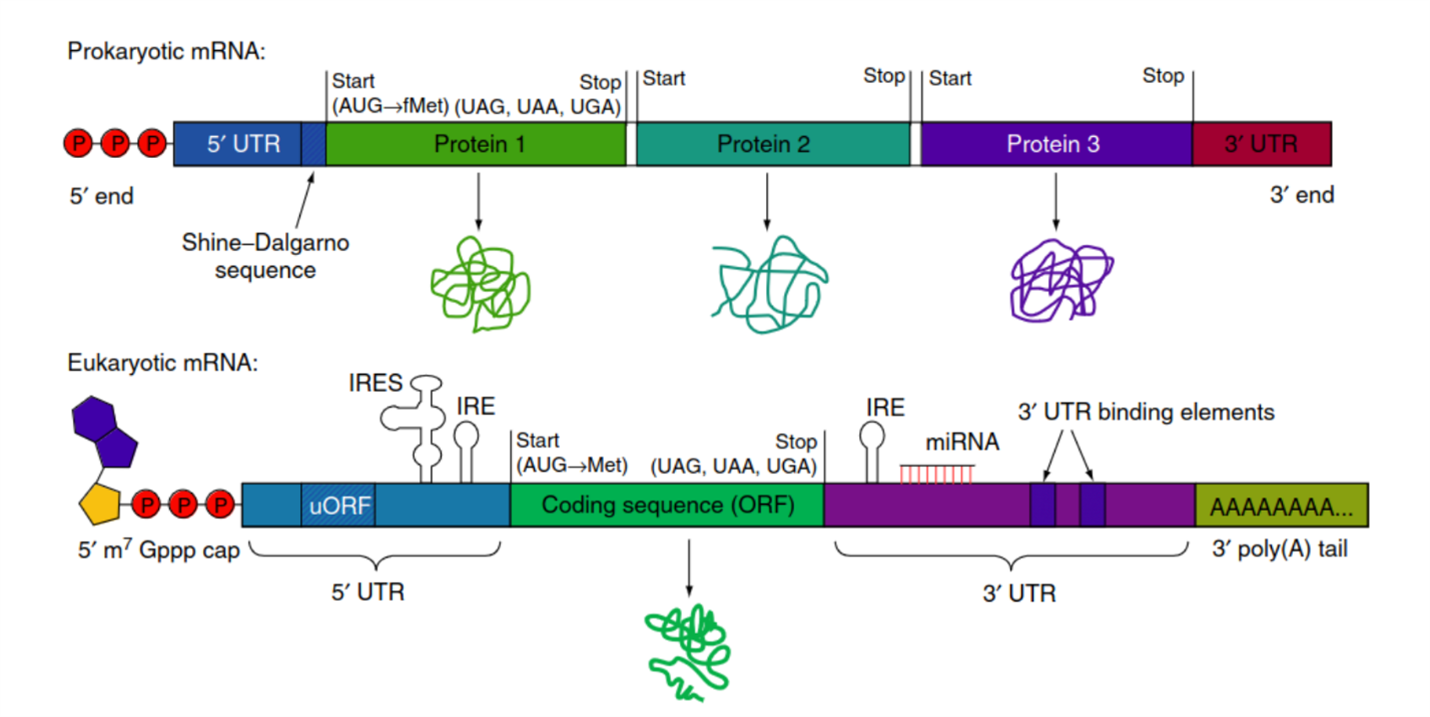
\includegraphics[width=1\linewidth]{./figure/mrna_comparison.png}
    \caption{Schematic diagram of prokaryotic (top) and eukaryotic (bottom) mRNA. Bars indicate the relative length of the regions. 
    Borrowed from \citetitle{Goss2016} \cite{Goss2016}.}
    \label{fig:mrna_comparison}
\end{figure}

\section{Prokaryotic vs Eukaryotic mRNA}
\subsection{Common structures}
The structures of both eukaryotic and prokaryotic genes involve several nested sequence elements. Each element has a specific 
function in the multi-step process of gene expression. The sequences and lengths of these elements vary, but the same general 
functions are present in most genes. Although DNA is a double-stranded molecule, typically only one of the strands encodes 
information that the RNA polymerase reads to produce protein-coding mRNA or non-coding RNA. This 'sense' or 'coding' strand, 
runs in the 5' to 3' direction where the numbers refer to the carbon atoms of the backbone's ribose sugar. The open reading frame (ORF) 
of a gene is therefore usually represented as an arrow indicating the direction in which the sense strand is read.  

Regulatory sequences are located at the extremities of genes. These sequence regions can be next to the transcribed region 
(the promoter) or separated by many kilobases (enhancers and silencers). The promoter is located at the 5' end of the gene 
and is composed of a core promoter sequence and a proximal promoter sequence. The core promoter marks the start site for 
transcription by binding RNA polymerase and other proteins necessary for copying DNA to RNA. The proximal promoter region 
binds transcription factors that modify the affinity of the core promoter for RNA polymerase. Genes may be regulated by 
multiple enhancer and silencer sequences that further modify the activity of promoters by binding activator or repressor 
proteins. Enhancers and silencers may be distantly located from the gene, many thousands of base pairs away. The binding 
of different transcription factors, therefore, regulates the rate of transcription initiation at different times and in 
different cells.  

Regulatory elements can overlap one another, with a section of DNA able to interact with many competing activators and repressors 
as well as RNA polymerase. For example, some repressor proteins can bind to the core promoter to prevent polymerase binding. For 
genes with multiple regulatory sequences, the rate of transcription is the product of all of the elements combined. Binding of 
activators and repressors to multiple regulatory sequences has a cooperative effect on transcription initiation.  

Although all organisms use both transcriptional activators and repressors, eukaryotic genes are said to be 'default off', 
whereas prokaryotic genes are 'default on'. The core promoter of eukaryotic genes typically requires additional activation 
by promoter elements for expression to occur. The core promoter of prokaryotic genes, conversely, is sufficient for strong 
expression and is regulated by repressors.

An additional layer of regulation occurs for protein coding genes after the mRNA has been processed to prepare it for 
translation to protein. Only the region between the start and stop codons encodes the final protein product. The flanking 
untranslated regions (UTRs) contain further regulatory sequences. The 3' UTR contains a terminator sequence, which marks 
the endpoint for transcription and releases the RNA polymerase. The 5' UTR binds the ribosome, which translates the 
protein-coding region into a string of amino acids that fold to form the final protein product. In the case of genes for 
non-coding RNAs the RNA is not translated but instead folds to be directly functional.

\subsection{Eukaryotes}
The structure of eukaryotic genes includes features not found in prokaryotes. Most of these relate to post-transcriptional 
modification of pre-mRNAs to produce mature mRNA ready for translation into protein. Eukaryotic genes typically have more 
regulatory elements to control gene expression compared to prokaryotes. This is particularly true in multicellular eukaryotes, 
including humans, where gene expression varies widely among different tissues.  

A key feature of the structure of eukaryotic genes is that their transcripts are typically subdivided into exon and intron 
regions. Exon regions are retained in the final mature mRNA molecule, whereas intron regions are excised during post-transcriptional 
processing. Indeed, the intron regions of a gene can be considerably longer than the exon regions. Once spliced together, 
the exons form a single continuous protein-coding region, and the splice boundaries are not detectable. Eukaryotic 
post-transcriptional processing also adds a 5' cap to the start of the mRNA and a poly-adenosine tail to the end of the mRNA. 
These additions stabilise the mRNA and direct its transport from the nucleus to the cytoplasm, although neither of these 
features are directly encoded in the structure of a gene.

\begin{figure}[!ht]
    \centering
    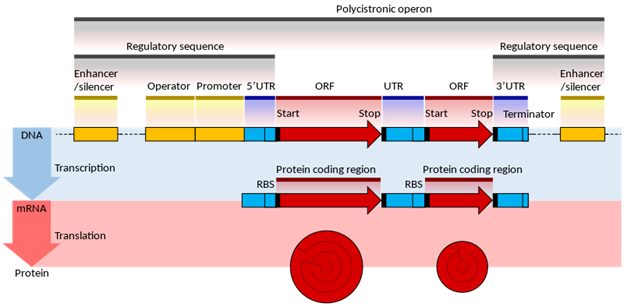
\includegraphics[width=1\linewidth]{./figure/eukaryote_mrna.png}
    \caption{The structure of a eukaryotic protein-coding gene. Regulatory sequence controls when and where expression occurs 
    for the protein coding region (red). Promoter and enhancer regions (yellow) regulate the transcription of the gene into a 
    pre-mRNA which is modified to remove introns (light grey) and add a 5' cap and poly-A tail (dark grey). The mRNA 5' and 3' 
    untranslated regions (blue) regulate translation into the final protein product. Borrowed from \citetitle{Schafee2017} \cite{Schafee2017}.}
    \label{fig:eukaryote_mrna}
\end{figure}

\subsection{Prokaryotes}
The overall organisation of prokaryotic genes is markedly different from that of the eukaryotes. The most obvious difference 
is that prokaryotic ORFs are often grouped into a polycistronic operon under the control of a shared set of regulatory sequences. 
These ORFs are all transcribed onto the same mRNA and so are co-regulated and often serve related functions. Each ORF typically 
has its own ribosome binding site (RBS) so that ribosomes simultaneously translate ORFs on the same mRNA. Some operons 
also display translational coupling, where the translation rates of multiple ORFs within an operon are linked. This can 
occur when the ribosome remains attached at the end of an ORF and simply translocates along to the next without the need 
for a new RBS. Translational coupling is also observed when translation of an ORF affects the accessibility of the next 
RBS through changes in RNA secondary structure. Having multiple ORFs on a single mRNA is only possible in prokaryotes because 
their transcription and translation take place at the same time and in the same subcellular location \cite{Schafee2017}.  

The operator sequence next to the promoter is the main regulatory element in prokaryotes. Repressor proteins bound to the 
operator sequence physically obstruct the RNA polymerase enzyme, preventing transcription. Riboswitches are other important 
regulatory sequences commonly present in prokaryotic UTRs. These sequences switch between alternative secondary structures 
in the RNA depending on the concentrations of key metabolites. The secondary structures then either block or reveal important 
sequence regions such as RBSs. Introns are extremely rare in prokaryotes and therefore do not play a significant role in 
prokaryotic gene regulation \cite{Schafee2017}.

\begin{figure}[!ht]
    \centering
    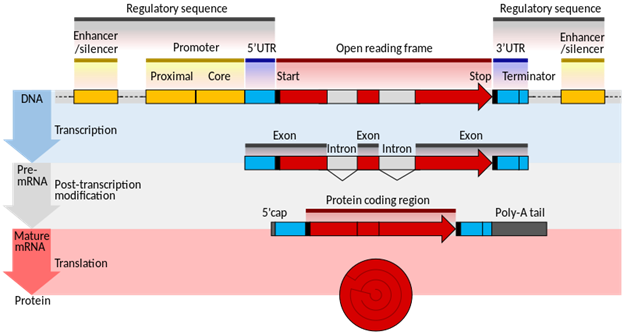
\includegraphics[width=1\linewidth]{./figure/prokaryote_mrna.png}
    \caption{The structure of a prokaryotic operon of protein-coding genes. Regulatory sequence controls when expression 
    occurs for the multiple protein coding regions (red). Promoter, operator and enhancer regions (yellow) regulate the 
    transcription of the gene into an mRNA. The mRNA untranslated regions (blue) regulate translation into the final protein 
    products. Borrowed from \citetitle{Schafee2017} \cite{Schafee2017}.}
    \label{fig:prokaryote_mrna}
\end{figure}

\begin{figure}[!ht]
    \centering
    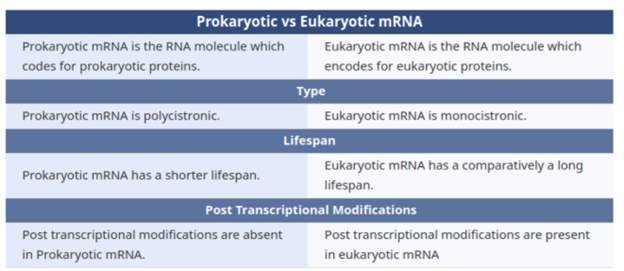
\includegraphics[width=1\linewidth]{./figure/mrna_comparison_table.png}
    \caption{Table comparison. Borrowed from somewhereelse.}
    \label{fig:mrna_comparison_table}
\end{figure}

\section{RNA-seq}
While a major challenge for early bacterial RNA-seq experiments was the presence of highly abundant RNA species like rRNAs 
and tRNAs, which make up more than 95\% of the RNA pool in a bacterial cell, this issue was overcome in eukaryotes by solely 
reverse-transcribing poly(A)-tailed mRNAs via oligo-d(T) priming during cDNA library preparation. Since poly(A)-tails represent 
a degradation signal in bacteria, several strategies for rRNA removal including oligonucleotide-based removal of rRNAs 
with magnetic beads or size fractionation using gel electrophoresis were employed  \cite{Bischler2015}.  

In a typical RNA-seq experiment total RNA or a fraction thereof is first converted into cDNA in a reverse-transcription 
reaction, followed by PCR-based amplification of the library. Different library protocols are available, which are highly 
specific for the applied sequencing technique but can be subdivided into strand-specific and non-strand-specific protocols. 
Non-strand-specific protocols, for example, based on random hexamer priming and ligation of adapters to double-stranded 
cDNA have the drawback that they lose the information whether sequencing reads originate from the sense or the antisense 
strand. To overcome this problem, strand-specific protocols have been developed including direct sequencing of first strand 
cDNA, template switching PCR, RNA C to U conversion using bisulfite or second strand synthesis with dUTP followed by degradation 
after adapter ligation \cite{Bischler2015,Sharma2014}.  

RNA-seq-based mapping of bacterial transcript boundaries enables a global elucidation of operon structures and facilitates 
annotation of untranslated regions (UTRs) of protein coding genes, which potentially contain gene regulatory elements. 
Additionally, it can improve genome annotation by providing extensive information on transcriptional start sites (TSS), 
untranslated regions (UTRs) of mRNA genes, and previously unknown open reading frames (ORFs) or sRNA genes \cite{Sharma2014}. 

\section{Differential RNA-seq}
Differential RNA-seq (dRNA-seq) method allows for global annotation of all expressed transcriptional start sites (TSS) under 
the examined growth condition in an organism of interest in one sequencing experiment. While it was originally developed to 
study the primary transcriptome of the major human pathogen Helicobacter pylori it has since been successfully applied for 
determination of TSS in a wide range of pro- and eukaryotic organisms. With >1900 unique TSS and at least one antisense TSS 
to 50\% of all genes, the dRNA-seq approach revealed a very complex and compact transcriptional output from the small 
\textit{H. pylori} genome and an unexpected number of \(\ge\)60 sRNA  \cite{Schafee2017}.

\begin{figure}[!ht]
    \centering
    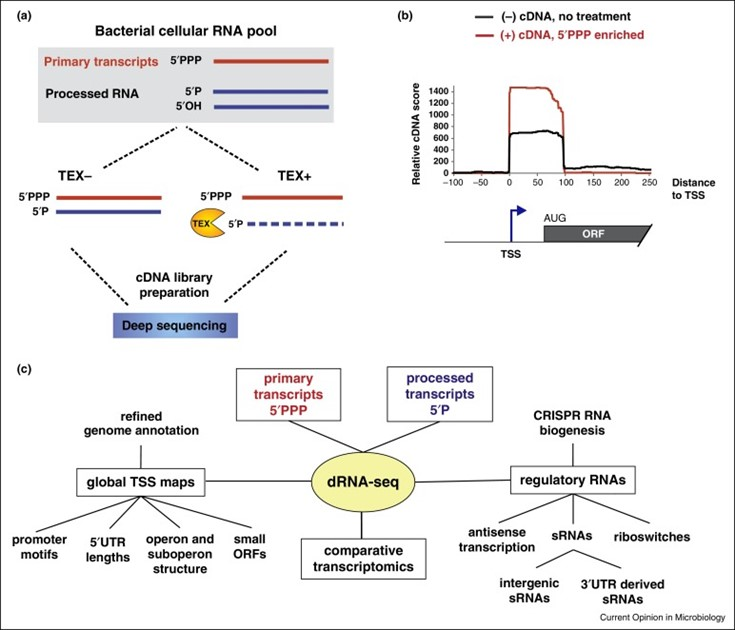
\includegraphics[width=1\linewidth]{./figure/dif_rnaseq.jpg}
    \caption{Rationale and output of the dRNA-seq approach. (a) Enrichment of primary transcripts using 5'-phosphate-dependent 
    terminator exonuclease (TEX). The bacterial RNA pool consists of primary transcripts with a 5'PPP and processed RNAs 
    with a 5'P or 5'OH. RNAs with a 5' OH group are not accessible for 5'-linker ligation during cDNA library constructions 
    and, thus, will not be represented in the cDNA library. For the construction of dRNA-seq libraries, each RNA sample is 
    split into two parts. One half remains untreated (TEX-), whereas the other half is treated with TEX which specifically 
    degrades RNAs with a 5' P, and thereby enriches for primary transcripts with a 5'PPP in relative terms. Upon differential 
    TEX treatment, both samples are converted into a cDNA library and analyzed by deep sequencing. (b) A dRNA-seq specific 
    cDNA enrichment pattern can be observed at the primary 5' ends of genes. Treatment with TEX (red curve; (+) library) 
    redistributes the cDNAs towards the nuclease-protected 5'-end, yielding a sawtooth-like profile with an elevated sharp 
    5' flank which can be used to annotate the TSS (blue arrow) of a gene of interest (grey bar). Note that dRNA-seq reads 
    cluster towards a gene's 5' end if no fragmentation is used. (c) Schematic summary of information that can be gained 
    from dRNA-seq to uncover transcriptome features and refine genome annotation. Borrowed from \citetitle{Sharma2014} \cite{Sharma2014}.}
    \label{fig:diff_rnaseq}
\end{figure}

\part{Metagenomics}
% !TEX root = ../notes_template.tex
\chapter{Metagenomics}\label{chp:metagenomics}

\minitoc

\section{Metagenomes reconstruction}
 
Binning. Critical step required to establish a genome from a metagenomic assembly. This involves assignment of assembled 
fragments to a draft genome based on detection on any scaffold of some signal(s) that occur(s) locally within a genome and 
persists genome-wide \cite{Chen2020}. 

Genome curation \cite{Hiltemann2023,microbiome-metagenomics-binning}. Filling scaffolding gaps and removal of local assembly 
errors. Gap filling strategies: 
\begin{itemize}
    \item[GapFiller] Tool for filling the N's gaps at scaffold joins. Often a few iterations are needed for gap closure. Using:
    \begin{itemize}
        \item Unplaced pairs for reads adjacent to the gaps. When reads are mapped to genome fragments that compose a bin, a 
        file of unplaced paired reads is generated for each fragment.
        \begin{itemize}
            \item If due to low coverage gap filling is not achieve, potentially use of reads from other sample in which the sample population occurs.
            \item Deeper sequencing of the same sample.
        \end{itemize}
        \item Placement of full metagenomic read data set to the new version of the scaffold.
        \item Use of misplaced reads. This can be useful in cases where the necessary reads are misplaced, either elsewhere 
        on that scaffold or on another scaffold in the bin. Misplaced read identification:
        \begin{itemize}
            \item Read pileups with anomalously high frequencies of SNVs in a subset of reads.
            \item Read pairs point outward (rather than toward each other, as expected).
            \item Unusually long paired read distances.
        \end{itemize}
        \item Sometimes even with sufficient read depth, gap filling cannot be achieved due to complex repeats. 
        Sometimes these repeat regions can be resolved careful read-by-read analysis, often requiring relocation of reads 
        based on the placement of their pairs and sequence identity.
    \end{itemize}
\end{itemize}

Local assembly errors (from more common to less):
\begin{itemize}
    \item Error I:
    \begin{description}
        \item[Identification] Sequence in that region lacks perfect support, by even one read.
        \item[Solution] Consensus sequence should be replaced by Ns (gap), which can be further filled.
        \item[Example] \url{https://genome.cshlp.org/content/suppl/2020/03/18/gr.258640.119.DC1/Supplemental_Fig_S3.pdf}.
    \end{description}  
    \item Error II:
    \begin{description}
        \item[Identification] Ns have been inserted during scaffolding despite overlap between the flanking sequences.
        \item[Solution] Close the gap, eliminating the Ns and the duplicated sequence.
        \item[Example] \url{https://genome.cshlp.org/content/suppl/2020/03/18/gr.258640.119.DC1/Supplemental_Fig_S4.pdf}.
    \end{description}
    \item Error III:
    \begin{description}
        \item[Identification] Incorrect number of repeats has been incorporated into the scaffold sequences. Anomalous read 
        depth over that region.
    \end{description}
    \item Error IV: Chimera sequences from two different organisms.
    \begin{description}
        \item[Identification] These joints typically lack paired read support and/or can be identified by very different 
        coverage values and/or phylogenetic profiles on either side of the join.
    \end{description}
    \item Error V: Artificial concatenation of an identical sequence.
    \begin{description}
        \item[Identification] Repeat finder.
    \end{description}
\end{itemize}

\section{Pangenomes}
[TO DO]
Differents genes within a population. Pangenome analysis.

\section{Microbila diversity}
[TO DO]
Beta diversity and its representation. Concept of dimensionality reduction techniques.

\section{Abundance estimation}
[TO DO]
How to quantify composition: markers genes and what makes good a marker gene (to be single and present in the core).

\section{Sequencing depth}
[TO DO]
Huttenhower -> For strain analysis = ideally 10X; Gene-absence: \(\backsim\)1X
Discoveries and findings with microbelix. 

\begin{appendices}
% !TEX root = ../notes_template.tex
\chapter{Formulas}

\section{Gaussian distribution}\label{sec:gaussian_distribution}
\begin{definition}[Gaussian distribution]\label{def:gaussian_distribution}
    \myindex{Gaussian distribution}
\end{definition}

\begin{theorem}[Central limit theorem]\label{thm:central_limit_theorem}
\end{theorem}
\end{appendices}

\backmatter

%%%%%%%%%%%%%%% Reference %%%%%%%%%%%%%%%

\printbibliography[heading=bibintoc]
\printindex

\end{document}

